\section{Case Studies}
\label{app:cases}
\suppressfloats[t]

This appendix presents ten case studies that show, on concrete programs, what symbolic execution contributes to generated specifications. Across all cases, \toolname\ reuses the same local symbolic context and template-routing signals, so each case emphasizes a distinct role of that context rather than repeating the full mechanism. Table~\ref{tab:case-study-map} summarizes the organization. The first five cases cover phase-split loop invariants, path-complete postconditions under C aliasing, recursive heap shape specifications, the contrast between RTE-safety and functional specification, and the scale boundary on industrial control code. The remaining five are supplementary evidence: the factorial and GCD cases show successful inductive-helper synthesis, MulLoop shows sign-sensitive invariant synthesis, Ackermann marks a recursion pattern beyond the current ACSL/SMT automation envelope, and matrix multiplication shows a verifier-timeout boundary rather than a generation failure. In the figures below, ACSL annotations enclosed by $/*@\cdots */$ are generated by \toolname\ and then retained after verification or pruning.

%Note that in all figures, the black boxes highlight the portions generated by the LLM, while the remaining elements are automatically derived through symbolic execution.

\begin{table}[H]
  \centering
  \caption{Organization of the case studies.}
  \label{tab:case-study-map}
  \begin{adjustbox}{max width=\linewidth}
  \begin{tabular}{lll}
    \toprule
    \textbf{Case} & \textbf{Location} & \textbf{Main lesson} \\
    \midrule
    SyGuS loop & Part I & Phase-split invariant from weak goals \\
    TripleAbsMax & Part I & Path-complete C/ACSL postconditions \\
    Linked list & Part I & Shape-predicate routing \\
    Linear search & Part I & RTE-safety vs.\ functional specification \\
    Industrial pipeline & Part I & Scale and verifier boundary \\
    Factorial, GCD & Part II & Inductive helper summaries \\
    MulLoop & Part II & Prior-tool contextual example \\
    Ackermann & Part II & ACSL/SMT recursion boundary \\
    Matrix multiply & Part II & Nested loops; verifier/SMT-timeout boundary \\
    \bottomrule
  \end{tabular}%
  \end{adjustbox}
\end{table}

\subsection{Case 1: Phase-Split Invariant from a Weak Goal}

\begin{figure}[!t]
    \centering
    \begin{tcolorbox}[casebox, title={Case 1: symbolic state exposes loop phases}]
\begin{lstlisting}[style=caseinnerstyle]
int unknown();

/*@ requires n > 0; */
void SyGuS38(int n) {
  int c = 0;

  /*@
    loop invariant ((c == 0)&&(n == \at(n,Pre))) || (1 <= c <= n) ;
    loop invariant n == \at(n,Pre);
    loop assigns c ;
  */
  while (unknown()) {
    if(c == n) {
      c = 1;
    }
    else {
      c = c + 1;
    }
  }

  /*@ assert (c == n) ==> (c >= 0); */
}
\end{lstlisting}
    \end{tcolorbox}
    \caption{Case 1 (SyGuS-38): a nondeterministic loop whose phase structure is exposed by symbolic execution.}
    \label{fig:case1}
\end{figure}

Fig.~\ref{fig:case1} isolates the benefit of symbolic execution when the assertion is too weak to guide invariant synthesis. The goal $(c = n) \Rightarrow (c \ge 0)$ can be proved by many uninformative invariants; what matters here is the loop's phase structure.

At the loop boundary, symbolic execution separates the unentered state (\texttt{c == 0}) from the inductive region (\texttt{1 <= c <= n}) and records that \texttt{n} is stable. The disjunctive template instantiates exactly that split, yielding an invariant that describes the loop behavior rather than merely satisfying the final assertion.

\subsection{Case 2: Path-Complete Postconditions \rev{for Pointer-Manipulating Code}}

\begin{figure}[!t]
    \centering
    \begin{tcolorbox}[casebox, title={\textcolor{white}{Case 2: path-complete postconditions for pointer-manipulating code}}, width=\linewidth]
\begin{lstlisting}[style=casecompactinnerstyle]
typedef struct __TripleAbsMax
{
  int abs[3];
  int tmax;
  int* ret;
} TripleAbsMax;

/*@
  requires \valid(pIp);
  requires \valid(pIp->abs+(0..2)) ;
  requires \valid(pIp->ret);
  requires \separated(pIp, pIp->ret);

  ensures pIp->ret == \old(pIp->ret);
  ensures -pIp->abs[2] <= pIp->abs[1] && pIp->abs[0] <= pIp->abs[1] && pIp->abs[2] < 0 && pIp->abs[1] >= 0
  && pIp->abs[0] >= 0 ==> pIp->tmax == pIp->abs[1] && *\old(pIp->ret) == pIp->abs[1];
  ... all 32 paths

  assigns pIp->tmax, *(pIp->ret);
*/
void TripleAbsMaxFun(TripleAbsMax *pIp)
{
  int absfx1 = pIp->abs[0];
  int absfy2 = pIp->abs[1];
  int absfz3 = pIp->abs[2];

  if (pIp->abs[0] < 0){  absfx1 = -pIp->abs[0];}

  if (pIp->abs[1] < 0){  absfy2 = -pIp->abs[1];}

  if (pIp->abs[2] < 0){  absfz3 = -pIp->abs[2];}

  if (absfx1 > absfy2){  pIp->tmax = absfx1;}
  else{ pIp->tmax = absfy2; }

  if (absfz3 > pIp->tmax){pIp->tmax = absfz3;}

  *(pIp->ret) = pIp->tmax;
}

/*@
  requires \valid(pIp);
  requires \valid(pIp->abs+(0..2));
  requires \valid(pIp->ret);
  requires \separated(pIp, pIp->ret);
*/
void main1(TripleAbsMax *pIp)
{
  pIp -> abs[0] = 1;
  pIp -> abs[1] = 2;
  pIp -> abs[2] = -3;

  TripleAbsMaxFun(pIp);

  /*@ assert pIp -> tmax == 3; */
}
\end{lstlisting}
    \end{tcolorbox}
    \caption{Case 2 (TripleAbsMax): \rev{a loop-free program with 32 feasible paths under the precondition shown.}}
    \label{fig:case3}
\end{figure}

Fig.~\ref{fig:case3}, from our \textbf{pIp} benchmark, is the main C-specific case. The function computes the maximum absolute value of three struct-stored integers and writes it both to \texttt{pIp->tmax} and through \texttt{pIp->ret}.

\rev{Starting from the default precondition, including \texttt{\textbackslash separated(pIp, pIp->ret)}, symbolic execution derives the guarded postconditions for the feasible paths.}
\subsection{Case 3: Shape-Predicate Routing for Linked Structures}

\begin{figure}[!t]
    \centering
    \begin{tcolorbox}[casebox, title={Case 3: route-selected shape predicates}]
\begin{lstlisting}[style=caseinnerstyle]
struct SLL {
    struct SLL *tail;
    int head;
};

/*@
  predicate lseg{L}(struct SLL* x, struct SLL* y) =
    x == y || (x != y && \valid(x) && \separated(x, y) && lseg{L}(x->tail, y));
*/

/*@ predicate listrep(struct SLL* head) = lseg(head, \null); */

/*@
  logic integer list_length{L}(struct SLL* x) =
    (x == \null) ? 0 : 1 + list_length{L}(x->tail);
*/

/*@
  requires listrep(l);
  requires \valid_read(&data);
  assigns \nothing;
  ensures listrep(l);
  ensures \result == l;
*/
struct SLL * main1(struct SLL *l, int data)
{
    struct SLL *p;
    p = l;

    /*@
      loop invariant listrep(p);
      loop invariant listrep(l);
      loop invariant lseg(l, p);
      loop invariant data == \at(data,Pre);
      loop invariant l == \at(l,Pre);
      loop invariant list_length(l) >= list_length(p);
      loop assigns p;
    */
    while (p) {
      if (p->head == data) {
        /*@ assert data == \at(data,Pre); */
        /*@ assert l == \at(l,Pre); */
        return l;
      }
      p = p->tail;
    }

    return l;
}
\end{lstlisting}
    \end{tcolorbox}
    \caption{Case 3 (linked-list traversal): a recursive data-structure program with shape predicates.}
    \label{fig:case4}
\end{figure}

Fig.~\ref{fig:case4} illustrates template routing rather than another scalar invariant pattern. The loop walks a singly linked list and returns the original head pointer, so ACSL needs an explicit heap-shape abstraction instead of only arithmetic facts.

Symbolic execution identifies \texttt{p} as the advancing list pointer and records the local update facts, while the static route recognizes the recursive type and field-access pattern. That route selects the recursive-shape template, which supplies \texttt{lseg}, \texttt{listrep}, and \texttt{list\_length}; the loop template then connects the original head to the current suffix through \texttt{lseg(l, p)}. The key point is that the shape predicates are injected through a program-structure route and then anchored by symbolic cursor facts, rather than invented from source text alone.

\subsection{Case 4: RTE Safety vs. Functional Specification}
\label{app:case-search}

We reuse the linear search example from Fig.~3 of Preguss~\cite{Wang2025ATO} and run \toolname\ on the same source. The point is not a head-to-head accuracy comparison: Preguss is driven by RTE-safety obligations, while \toolname\ attempts to generate goal-independent functional specifications. This distinction also affects failure handling. On the Frama-C validation side, \toolname\ records potential RTE reports as warnings rather than treating RTE elimination as the main target. On the QCP side, however, an RTE can still block symbolic execution; the flattened-memory default precondition covers validity, bounds, and separation facts exposed by the model, but it does not guarantee that every arithmetic or pointer-related RTE is avoided. The refinement stage can ask the LLM to strengthen preconditions to avoid such failures, but this is a supporting mechanism for functional specification generation rather than the objective itself.

\begin{figure}[!t]
  \centering
  \begin{tcolorbox}[casebox, title={Preguss: RTE-guided safety specification}, width=0.96\linewidth]
\begin{lstlisting}[style=casecompactinnerstyle]
/*@ requires \valid_read(arr+(0..len-1));
    assigns \nothing; */
int * search(int * arr, int len, int val) {
    int i = 0;
    /*@ loop assigns i; */
    while (i < len) { ... }
}
\end{lstlisting}
  \end{tcolorbox}
  \vspace{1.4ex}

  \begin{tcolorbox}[casebox, title={\toolname: verifier-checked prefix-search specification}, width=0.96\linewidth]
\begin{lstlisting}[style=casecompactinnerstyle]
/*@ logic integer count_eq{L}(int* a, integer lo,
      integer hi, integer v) =
      lo >= hi ? 0 : count_eq(a, lo, hi - 1, v)
                   + (a[hi - 1] == v ? 1 : 0); */
/*@ requires \valid(arr + (0 .. len - 1));
    requires len >= 0;
    ensures \forall integer k; 0 <= k < len ==>
              arr[k] == \at(arr[k], Pre);
    ensures \result == \null ==>
              count_eq(arr, 0, len, val) == 0;
    ensures \result != \null ==>
              count_eq(arr, 0, \result - arr, val) == 0
              && *\result == val;
    assigns \nothing; */
int * search(int * arr, int len, int val) {
    int i = 0;
    /*@ loop invariant 0 <= i <= len;
        loop invariant \forall integer k;
            0 <= k < len ==> arr[k] == \at(arr[k], Pre);
        loop invariant count_eq(arr, 0, i, val) == 0;
        loop assigns i; loop variant len - i; */
    while (i < len) {
        if (arr[i] == val) return arr + i;
        i = i + 1;
    }
    return (int *)0;
}
\end{lstlisting}
  \end{tcolorbox}
  \caption{Case 4 (linear search). Preguss verifies memory-access safety; \toolname\ also captures the prefix-search property and returned-pointer consequence.}
  \label{fig:case7}
\end{figure}

Fig.~\ref{fig:case7} shows the difference in target. Preguss emits the memory-safety precondition needed to discharge \texttt{arr[i]} accesses. \toolname\ instead routes the loop to a count-occurrences helper and records both return cases: null means \texttt{val} is absent, and non-null means the returned pointer dereferences to \texttt{val} with no earlier occurrence. This illustrates why RTE-safety synthesis of Preguss~\cite{Wang2025ATO} and our functional specification synthesis should not be read as identical tasks.

\subsection{Case 5: Industrial Pipeline Stress Test}
\label{subsec:case9-ip}

\begin{figure*}[!t]
    \centering
    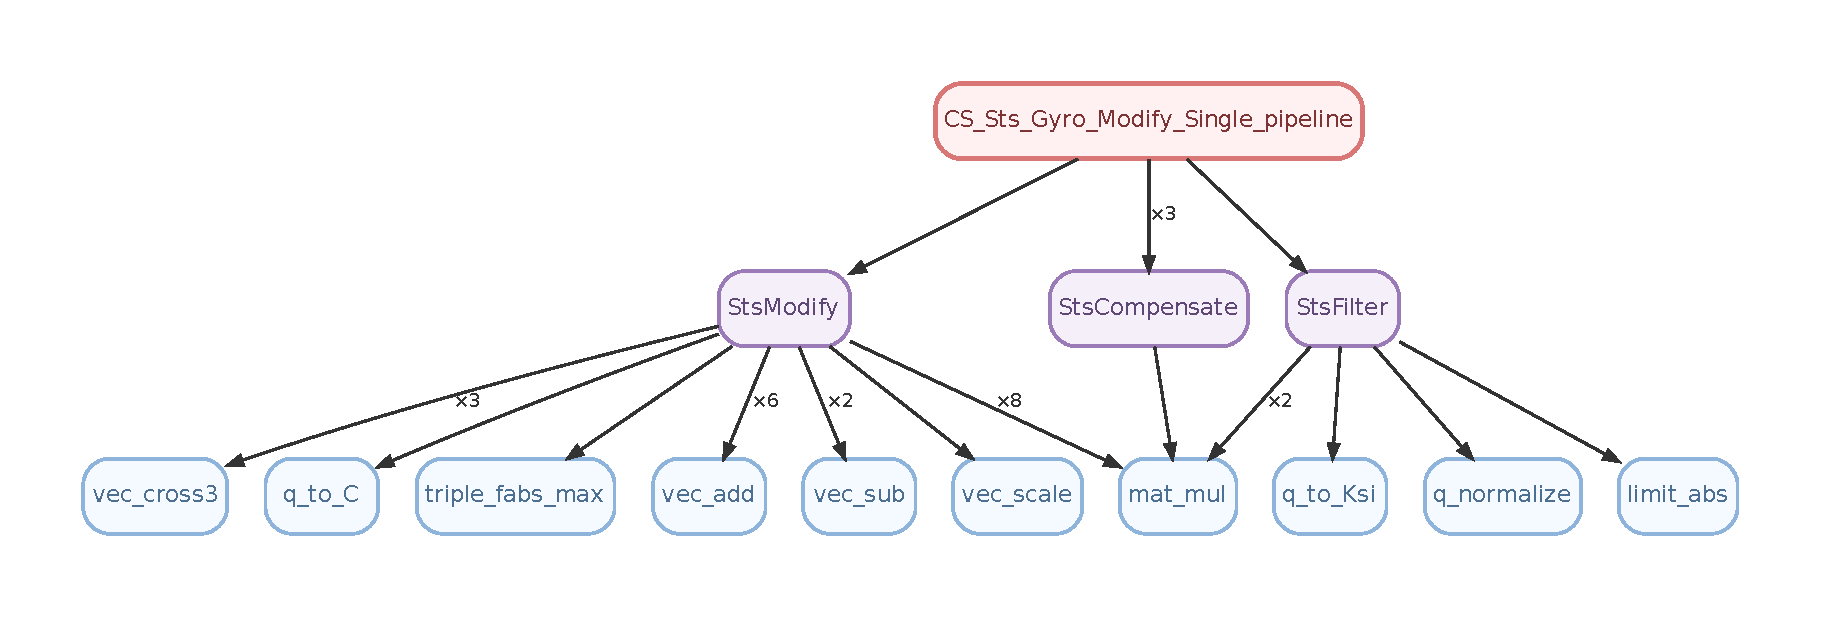
\includegraphics[width=0.95\textwidth]{images/ip_callgraph.pdf}
    \caption{Call graph of the single-star-sensor filter-update pipeline. Edge labels show call multiplicity; unlabeled edges are $\times 1$.}
    \label{fig:case9-callgraph}
\end{figure*}

\smallskip
\noindent\textbf{Program structure.}
We applied \toolname\ to a 225-line C transcription of an industrial single-star-sensor Kalman-update pipeline. The translation unit contains 14 functions, 33 call sites, and 8 loops; the entry delegates to three pipeline stages, which in turn call ten numeric and quaternion helpers (Fig.~\ref{fig:case9-callgraph}). This case is included to show the scale boundary, not another single function invariant pattern.

\smallskip
\noindent\textbf{What \toolname\ produced.}
Driven by \texttt{gpt-5.4-mini} at maximum reasoning effort (\texttt{reasoning\_effort=high}) in the goal-independent configuration, \rev{\toolname\ completed specification generation for 13 of the 14 functions.} The assembled file contains 198 ACSL clauses, and Frama-C/WP discharges 601 of 625 verification conditions ($96.2\%$) at a 30\,s per-goal timeout. Table~\ref{tab:case9-wp} shows that increasing the timeout from 5\,s to 30\,s recovers only one additional goal, so the residual failures reflect hard proof obligations rather than transient budget noise.

\rev{Because proof discharge alone does not measure specification informativeness, we also manually audited the accepted contract of each function. We count a postcondition as functional only when it gives a non-vacuous relation between the output or return value and the inputs; \texttt{ensures \textbackslash true} receives no such credit. Ten functions have functional postconditions: \texttt{limit\_abs}, \texttt{q\_to\_C}, \texttt{q\_to\_Ksi}, \texttt{triple\_fabs\_max}, \texttt{vec\_cross3}, \texttt{vec\_scale}, \texttt{vec\_add}, \texttt{vec\_sub}, \texttt{StsCompensate}, and \texttt{StsFilter}. The other four lack a complete functional summary: \texttt{StsModify} provides only output bounds, \texttt{mat\_mul} has the vacuous \texttt{ensures \textbackslash true}, and the no-op helper \texttt{q\_normalize} and the top-level \texttt{CS\_Sts\_Gyro\_Modify\_Single\_pipeline} have no explicit accepted contract.}

\begin{table}[!t]
  \centering
  \caption{Frama-C/WP proof obligations for the aerospace pipeline.}
  \label{tab:case9-wp}
  \begin{tabular}{lrrr}
    \toprule
    & \multicolumn{3}{c}{\textbf{per-goal timeout}} \\
    \cmidrule(lr){2-4}
    \textbf{Disposition} & \textbf{5\,s} & \textbf{10\,s} & \textbf{30\,s} \\
    \midrule
    Total       & 625           & 625           & 625           \\
    Valid       & 600           & 601           & 601           \\
    Unknown     & 2             & 2             & 3             \\
    Timeout     & 23            & 22            & 21            \\
    \midrule
    Discharge rate & $96.0\%$ & $96.2\%$ & $96.2\%$ \\
    \bottomrule
  \end{tabular}
\end{table}

\smallskip
\noindent\textbf{Boundary exposed.}
\rev{The functions with functional summaries are mostly arithmetic leaves whose semantics admit closed-form ACSL relations, such as \texttt{limit\_abs}, \texttt{vec\_cross3}, and \texttt{q\_to\_C}.} The hard cases are delegate functions and matrix-style loops: composing multi-stage callee summaries and expressing row-major matrix products require either user-provided logic summaries or proof automation beyond the current SMT-only backend. \rev{Thus the $96.2\%$ discharge rate measures verifier acceptance of the generated annotations, while the contract audit separately exposes how much functional behavior those annotations capture.} Concretely, the undischarged goals concentrate in the matrix-multiply leaf \texttt{mat\_mul} and its callers, exactly the triple-nested product dissected in the supplementary matrix-multiplication case below, where the recursive \texttt{mat\_sum} over nonlinear indices makes Z3 time out and the accepted specification degrades to \texttt{ensures \textbackslash true}.

\subsection{Supplementary Cases}

\Needspace*{10\baselineskip}
\paragraph{Factorial: Guarded Inductive Helper.}
\label{app:case-factorial}

\begin{figure}[!b]
    \centering
    \begin{tcolorbox}[casebox, title={Supplementary Case: guarded factorial helper}, width=\linewidth]
\begin{lstlisting}[style=casecompactinnerstyle]
int unknown();

/*@
  logic integer product(integer begin, integer end) =
    (end < begin) ? 1 : product(begin, end - 1) * end;
*/

/*@
  requires \true;
  assigns \nothing;
  ensures (n < 1) ==> \result == 1;
  ensures (n >= 1) ==> \result == product(1, n);
*/
int factorial9(int n) {
  int i = 1;
  int f = 1;

  /*@
    loop invariant (1 <= \at(n,Pre)) ==> (1 <= i <= n + 1);
    loop invariant (1 <= \at(n,Pre)) ==> (f == product(1, i - 1));
    loop invariant (!(1 <= \at(n,Pre))) ==> ((f == 1)&&(i == 1)&&(n == \at(n,Pre)));
    loop invariant n == \at(n,Pre);
    loop assigns f, i;
  */
  while (i <= n) {
    f = f * i;
    i = i + 1;
  }

  return f;
}

void goo9() {
  int t = factorial9(5);
  //@ assert t == 120;
}
\end{lstlisting}
    \end{tcolorbox}
    \caption{Supplementary factorial case: a guarded loop invariant with a recursive \texttt{product} helper.}
    \label{fig:case2}
\end{figure}

Fig.~\ref{fig:case2} complements the phase-split loop case (Case 1) above: the loop may be skipped when \texttt{n < 1}, and the entered region requires the inductive relation \texttt{f == product(1, i - 1)}. Symbolic execution provides the entered/unentered guard, while the static route selects the inductive-helper template that supplies the ACSL \texttt{product} definition used by both the invariant and the postcondition.

\Needspace*{10\baselineskip}
\paragraph{GCD: Recursive Summary with a Simple Measure.}
\label{app:case-gcd}

\begin{figure}[!b]
    \centering
    \begin{tcolorbox}[casebox, title={Supplementary Case: recursive GCD summary}]
\begin{lstlisting}[style=casecompactinnerstyle]
/*@ 
  logic integer gcd_logic(integer a, integer b) =
    (a == 0) ? b :
    (b == 0) ? a :
    (a == b) ? a :
    (a > b) ? gcd_logic(a - b, b) :
               gcd_logic(a, b - a);
*/

/*@
requires \true;
decreases a + b;
assigns \nothing;
ensures \result == gcd_logic(a, b);
*/
int gcd(int a, int b) 
{
    if (a == 0)
       return b;

    if (b == 0)
       return a;

    if (a == b)
        return a;

    if (a > b)
        return gcd(a-b, b);
    return gcd(a, b-a);
}

int main2()
{
    int a = 98, b = 56;
    int c = gcd(a, b);
    //@ assert c == 14;
    return 0;
}
\end{lstlisting}
    \end{tcolorbox}
    \caption{Supplementary recursive GCD case: a recursive logic summary with a single arithmetic termination measure.}
    \label{fig:case5}
\end{figure}

Fig.~\ref{fig:case5} shows the recursion case where the current workflow succeeds cleanly. When symbolic execution reaches a recursive call, \toolname\ switches to the recursion template, emits \texttt{gcd\_logic} branch-by-branch, and uses \texttt{decreases a + b}. This case is useful mainly as a contrast to the Ackermann case below: GCD needs only a single-measure descent and a single-unfold style of reasoning.

\Needspace*{10\baselineskip}
\paragraph{MulLoop: Signed Multiplication Loop.}
\label{app:case-mulloop}

\begin{figure}[!b]
    \centering
    \begin{tcolorbox}[casebox, title={Supplementary Case: signed multiplication loop}]
\begin{lstlisting}[style=casecompactinnerstyle]
int foo57(int a, int b);

/*@
  requires \true;
  assigns \nothing;
  ensures \result == a * b;
*/
int foo57(int a, int b) {
    int res = 0;
    if (b >= 0) {
        /*@
          loop invariant 0 <= i <= b;
          loop invariant res == i * a;
          loop assigns i, res;
          loop variant b - i;
        */
        for (int i = 0; i < b; i++) {
            res = res + a;
        }
    } else {
        /*@
          loop invariant 0 <= i <= -b;
          loop invariant res == -i * a;
          loop assigns i, res;
          loop variant -b - i;
        */
        for (int i = 0; i < -b; i++) {
            res = res - a;
        }
    }
    return res;
}
\end{lstlisting}
    \end{tcolorbox}
    \caption{Supplementary MulLoop case from \textbf{SpecGenBench}.}
    \label{fig:case6}
\end{figure}

Fig.~\ref{fig:case6} computes $a \cdot b$ by addition or subtraction depending on the sign of \texttt{b}. The negative branch requires the asymmetric invariant \texttt{res == -i * a}; reusing the positive-branch form would make the functional postcondition fail. In our run, \toolname\ retains \texttt{ensures \textbackslash result == a * b} because the branch condition selects the correct invariant template.

\Needspace*{10\baselineskip}
\paragraph{Ackermann: Recursion Beyond ACSL/SMT Automation.}
\label{app:case-ackermann}

\begin{figure}[!b]
    \centering
    \begin{tcolorbox}[casebox, title={Supplementary Case: Ackermann recursion boundary}]
\begin{lstlisting}[style=casecompactinnerstyle]
int foo1(int m, int n);

/*@
  logic integer ackermann(integer m, integer n) =
    (m == 0) ? n + 1 :
    (n == 0) ? ackermann(m - 1, 1) :
               ackermann(m - 1, ackermann(m, n - 1));
*/

/*@
  requires m >= 0 && n >= 0;
  decreases m * 1000 + n;
  assigns \nothing;
  ensures \result == ackermann(m, n);
*/
int foo1(int m, int n) {
    if (m == 0) {
        return n + 1;
    }
    if (n == 0) {
        return foo1(m - 1, 1);
    }
    return foo1(m - 1, foo1(m, n - 1));
}
\end{lstlisting}
    \end{tcolorbox}
    \caption{Supplementary Ackermann case. The candidate specification is syntactically clean but not discharged by Frama-C/WP under the current ACSL/SMT backend.}
    \label{fig:case8}
\end{figure}

Fig.~\ref{fig:case8} marks a boundary rather than a prompt failure. The generated helper follows the C branch structure, but Ackermann needs a lexicographic termination argument and nested induction that are not handled well by the current ACSL/SMT stack. A scalar \texttt{decreases m * 1000 + n} is not a sound substitute for the true lexicographic descent once \texttt{n} grows, and the functional postcondition would require proof support beyond the single-unfold reasoning that succeeds for GCD.

\Needspace*{10\baselineskip}
\paragraph{Matrix Multiplication: Triple-Nested Loops Beyond Per-Loop Symbolic Context.}
\label{app:case-matmul}

\begin{figure}[!b]
    \centering
    \begin{tcolorbox}[casebox, title={Supplementary Case: matrix-multiplication proof boundary}, width=\linewidth]
\begin{lstlisting}[style=casecompactinnerstyle]
/*@
  logic integer mat_sum(int *A, int *B, integer ca_rb, integer cb,
                        integer i, integer j, integer k) =
    k <= 0 ? 0 :
    mat_sum(A, B, ca_rb, cb, i, j, k - 1) +
    A[i * ca_rb + (k - 1)] * B[(k - 1) * cb + j];
*/

/*@
  requires \valid(out + (0 .. ra*cb - 1));
  requires \valid(A   + (0 .. ra*ca_rb - 1));
  requires \valid(B   + (0 .. ca_rb*cb - 1));
  requires \separated(out + (0..ra*cb-1), A + (0..ra*ca_rb-1));
  requires \separated(out + (0..ra*cb-1), B + (0..ca_rb*cb-1));
  // default precondition also bounds every cell to [0,100] and each
  // dimension product to (0,100), keeping the arithmetic overflow-free
  assigns out[0 .. ra*cb - 1];
  ensures \forall integer i, j; 0 <= i < ra && 0 <= j < cb ==>
      out[i*cb + j] == mat_sum(A, B, ca_rb, cb, i, j, ca_rb); // Z3 TIMEOUT (10s)
*/
void mat_mul(int *out, int *A, int *B, int ra, int ca_rb, int cb) {
  /*@
    loop invariant 0 <= i <= ra;
    loop invariant \forall integer ii, jj; 0 <= ii < i && 0 <= jj < cb ==>
        out[ii*cb + jj] == mat_sum(A, B, ca_rb, cb, ii, jj, ca_rb); // Z3 TIMEOUT (10s)
    loop invariant \forall integer p; i*cb <= p < ra*cb ==> out[p] == \at(out[p],Pre); // Z3 TIMEOUT
    loop assigns i, out[0 .. ra*cb - 1];
  */
  for (int i = 0; i < ra; i++) {
    /*@
      loop invariant 0 <= j <= cb;
      loop invariant \forall integer jj; 0 <= jj < j ==>
          out[i*cb + jj] == mat_sum(A, B, ca_rb, cb, i, jj, ca_rb); // Z3 TIMEOUT (10s)
      loop assigns j, out[i*cb .. i*cb + cb - 1];
    */
    for (int j = 0; j < cb; j++) {
      int s = 0;
      /*@
        loop invariant 0 <= k <= ca_rb;
        loop invariant s == mat_sum(A, B, ca_rb, cb, i, j, k); // DISCHARGED (one-step induction)
        loop assigns k, s;
      */
      for (int k = 0; k < ca_rb; k++)
        s = s + A[i*ca_rb + k] * B[k*cb + j];
      out[i*cb + j] = s;
    }
  }
}
\end{lstlisting}
    \end{tcolorbox}
    \caption{Supplementary matrix-multiplication case ($\mathit{ra}\times\mathit{ca\_rb}$ by $\mathit{ca\_rb}\times\mathit{cb}$ product). \toolname\ generates the correct quantified specification, but Frama-C/WP$\rightarrow$Z3 times out on the outer invariants and postcondition, so the accepted specification degrades to \texttt{ensures \textbackslash true}.}
    \label{fig:case-matmul}
\end{figure}

Fig.~\ref{fig:case-matmul} is the multi-loop boundary that Reviewer~2's failure-case question targets. \toolname\ emits the intended quantified postcondition and the matching outer-loop invariants, while the innermost \texttt{s == mat\_sum(\dots,k)} invariant is discharged by one-step induction. The remaining quantified obligations time out in Z3 because they combine recursive logic unfolding, havoc-updated array memory, and non-linear index arithmetic; refinement therefore strips the unproved clauses and the accepted specification collapses to verifier-valid but vacuous \texttt{ensures \textbackslash true}. This case illustrates a proof-automation limit rather than a generation failure.
